\documentclass[10pt,pdf,aspectratio=169]{beamer}
\usepackage[T2A]{fontenc}       %поддержка кириллицы
\usepackage[utf8]{inputenc}
\input{../../../../.preambles/20-math}
\newcommand{\ds}{\displaystyle}
\usepackage{graphicx}
\graphicspath{{plots/}}
%\usetheme{Hannover}
\usetheme{Singapore}
\usefonttheme{structurebold}
\usefonttheme[onlymath]{serif}
\setbeamercovered{transparent}

\title[Отбор одного из равноправных]{Мультистационарные системы. Отбор одного
из равноправных}
\author[]{Чечеткин~И.~А.}
\date{}

\begin{document}
\begin{frame}[plain]
\maketitle
\end{frame}

\section{Отбор одного из равноправных в отсутствии ограничений роста}
\begin{frame}
    \frametitle{Отбор одного из равноправных}
    \[
        \der{X_i}{t} = bX_i - \gamma\sum_{\substack{j = 1 \\ j \ne i}}^N X_i
        X_j \quad \bigr(i = 1, 2, \ldots, N\bigl).
    \]
\end{frame}
\begin{frame}
    \frametitle{Отбор одного из двух равноправных}
        \visible<1->{\[
            \der{X}{t} = bX - \gamma XY, \quad \der{Y}{t} = bY - \gamma XY
        \]}
        \visible<2->{\[
            t' = bt; \ x = \gamma X/b; \ y = \gamma Y/b
        } \visible<3->{
            .\quad \der{x}{t'} = x - xy; \quad \der{y}{t'} = y - xy
        \]}
        \visible<4->{\[
            x - xy = 0,\ y - xy = 0\colon \quad \bar{x}_1 = \bar{y}_1 = 0,\ 
            \bar{x}_2 = \bar{y}_2 = 1
        \]}
        \visible<5->{\[
            \bar{X}_1 = \bar{Y}_1 = 0;\ \ \bar{X}_2 = \bar{Y}_2 =
            \frac{b}{\gamma}
        } \visible<6->{
            ;\ \ \bar{X}_3\to\infty,\ \bar{Y}_3\to 0;\ \ \bar{X}_4\to 0,\ 
            \bar{Y}_4\to\infty
        \]}
\end{frame}
\begin{frame}
    \begin{figure}
        \center
        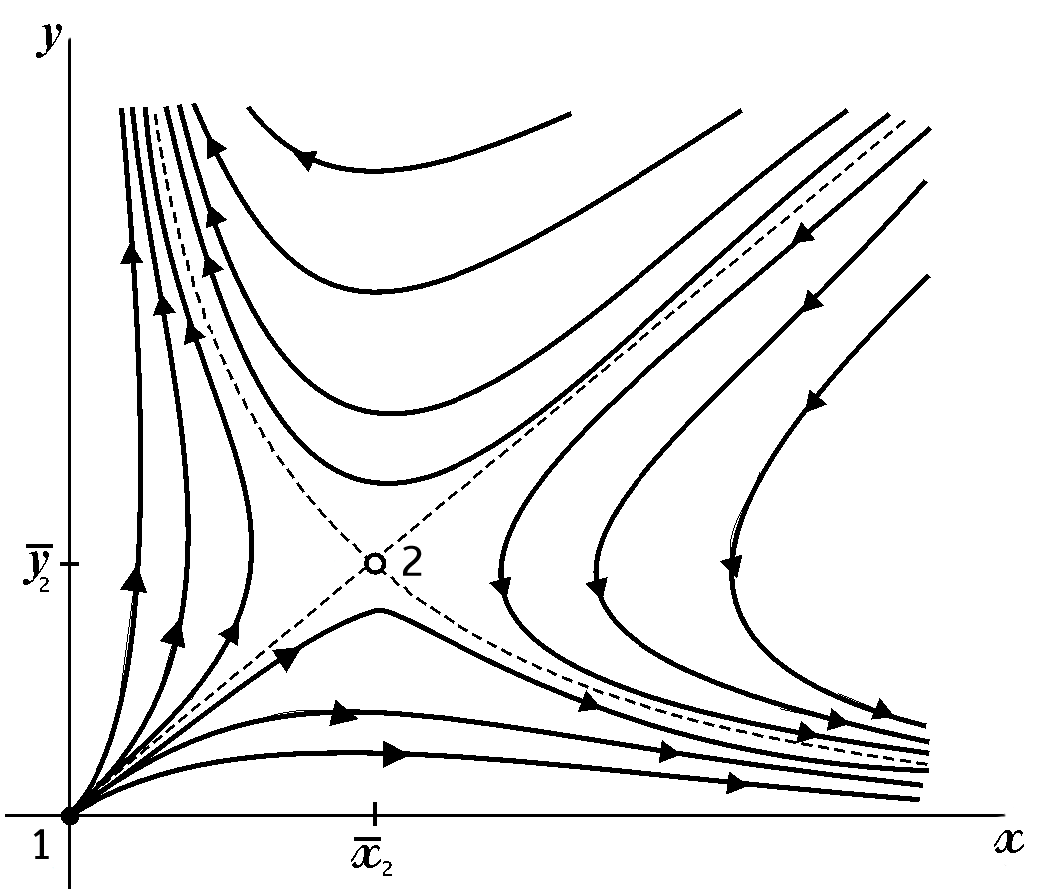
\includegraphics[width=.7\textheight]{one_of_two_unlimited}
    \end{figure}
\end{frame}
\begin{frame}
    \frametitle{Отбор одного из нескольких равноправных}
    \visible<1->{\[
        \der{X_i}{t} = bX_i - \gamma\sum_{j=1}^N X_iX_j + \gamma X_i^2, \quad
        \bigr(i = 1, 2, \ldots, N\bigl)
    \]}
    \visible<2->{\[
        t' = bt; \ x_i = \gamma X_i/b
    \]}
    \visible<3->{\[
        \der{x_i}{t'} = x_i\left( 1 - \sum_{j = 1}^N x_j \right) + x_i^2 \quad
        \bigl(i = 1, 2, \ldots, N\bigr)
    \]}
    \visible<4->{\[
        \bar{x}_i = 0;\ \ \bar{x}_i = (N - 1)^{-1}
    } \visible<5->{
        ;\ \ \bar{x}_i\to\infty,\ \bar{x}_j\to 0, \ \big(i, j \in [1, N],\ j \ne i\big)
    \]}
\end{frame}
\section{Отбор одного из равноправных при ограниченном субстрате}
\begin{frame}
    \frametitle{Отбор одного из равноправных при ограниченном субстрате}
    \visible<1->{\[
        a = \frac{a_0 S}{K_S + S}
    \]}
    \visible<2->{\[
        \only<3->{\left\{ }\begin{array}{l}
            \ds \der{S}{t} = -\alpha a(X + Y) + v = -\alpha a_0
            \frac{S}{K_S + S} + v \\[.7em]
        } \visible<3->{
            \ds \der{X}{t} = a_0\frac{S}{K_S + S}X - \beta X - \gamma XY, \\[.7em]
            \ds \der{Y}{t} = a_0\frac{S}{K_S + S}Y - \beta Y - \gamma XY,
        \end{array}} \only<3->{\right.}
    \]
    \visible<4->{\[
        t' = \beta t,\ x = \gamma X/\beta,\ y = \gamma Y/\beta,\ s = \gamma
        S/\beta,\ v' = v\gamma/\beta^2
    } \visible<5->{
        ,\ k_s = \gamma K_S/\beta,\ f(s) = a_0s/\beta(k_s + s)
    \]}
    \visible<6->{\[
        \left\{ \begin{array}{l}
            \ds \der{x}{t'} = f(s)x - x - xy, \\[.7em]
            \ds \der{y}{t'} = f(s)y - y - xy, \\[.7em]
            \ds \der{s}{t'} = -\alpha f(s)(x + y) + v'.
        \end{array} \right.
    \]}
\end{frame}
\begin{frame}
    \visible<1->{\[
         v' \gg 1, \quad \alpha \gg 1
    \]}
    \visible<2->{\[
        \invisible<3->{
            \der{s}{t'}\!\!
        } \only<3->{
            \invisible<4->{
                0\!\!
             }
        }
        \visible<4->{
            v'
        } = \invisible<4->{
            -
        } \only<4->{
            \!\!\!\!\!\!\!
        } \alpha f(s)(x + y) \invisible<4->{
            + v'
        } \visible<5->{
             \qquad f(s) = \frac{v'}{\alpha(x + y)}
        }
    \]}
    \visible<6->{\[
        \left\{ \begin{array}{l}
            \ds \der{x}{t'} = x\left[\frac{v_0}{x + y} - (1 + y)\right], \\[1em]
            \ds \der{y}{t'} = y\left[\frac{v_0}{x + y} - (1 + x)\right].
        \end{array} \right.
        \qquad v_0 = v'/\alpha
    \]}
    \visible<7>{\[
        \bar{x}_1 = \bar{y}_1 = 0;\ \ \bar{x}_2 = 0, \bar{y}_2 = v_0;\ \ 
        \bar{x}_3 = v_0, \bar{y}_3 = 0;\ \ \bar{x}_4 = \bar{y}_4 =
        \frac{\sqrt{1 + 2v_0} - 1}{2}
    \]}
\end{frame}
\begin{frame}
    \begin{figure}
        \center
        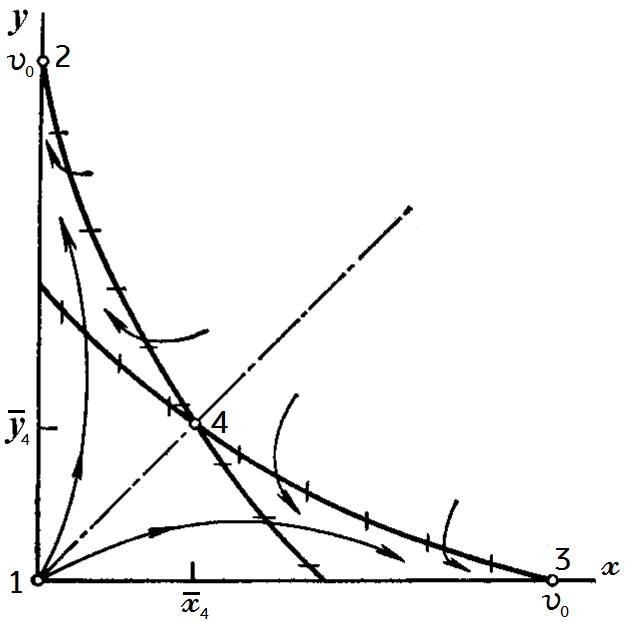
\includegraphics[width=.7\textheight]{one_of_two_limited}
    \end{figure}
\end{frame}
\end{document}
